% *******************************************************************************
% * Copyright (c) 2007 by Elexis
% * All rights reserved. This document and the accompanying materials
% * are made available under the terms of the Eclipse Public License v1.0
% * which accompanies this distribution, and is available at
% * http://www.eclipse.org/legal/epl-v10.html
% *
% *  $Id: agenda.tex 4904 2009-01-03 17:58:33Z rgw_ch $
% *******************************************************************************
% !Mode:: "TeX:UTF-8" (encoding info for WinEdt)

\section{Agenda de Elexis}\label{Agenda}
\index{rendez-vous} Il s'agit d'une agenda multiposte pour plusieurs mandants. Ce Plugin fait parti de la distribution standard. Ce qui suit explique la configuration et l'utilisation de l'agenda.
\subsection{Configuration}


Choisissez dans le menu  \textbf{Fichier -Options}. Si le Plugin Agenda est installé, vous trouverez là une rubrique  \textit{Agenda}:



%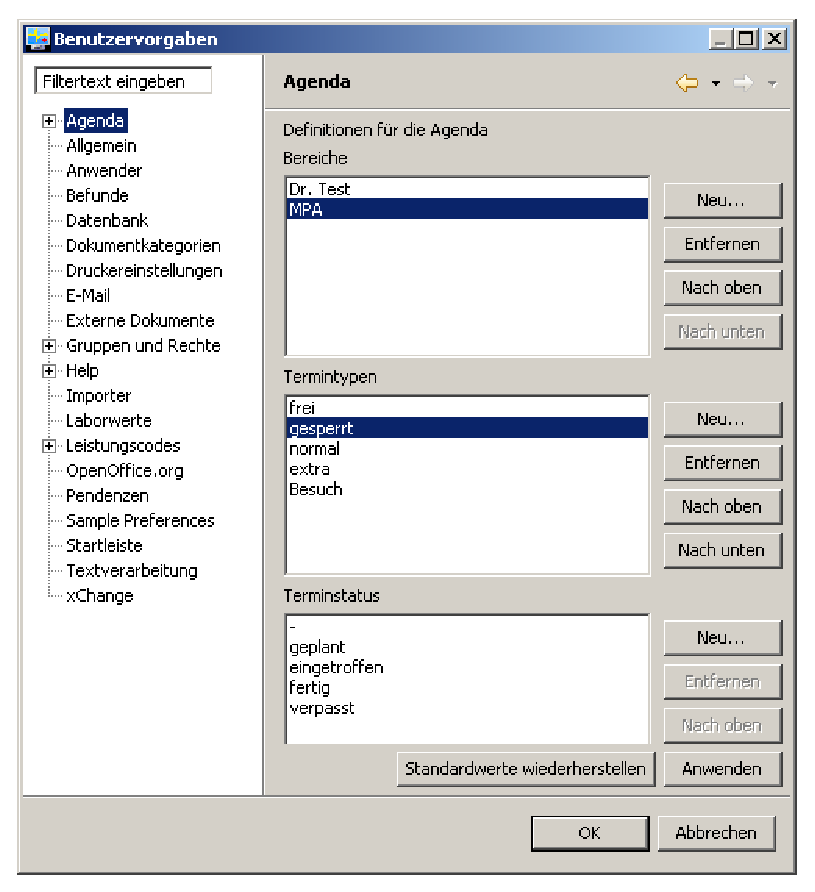
\includegraphics[width=3in,bb=0 0 382 420]{images/settings1}
% settings1.jpg: 499x548 pixel, 94dpi, 13.49x14.81 cm, bb=0 0 382 420

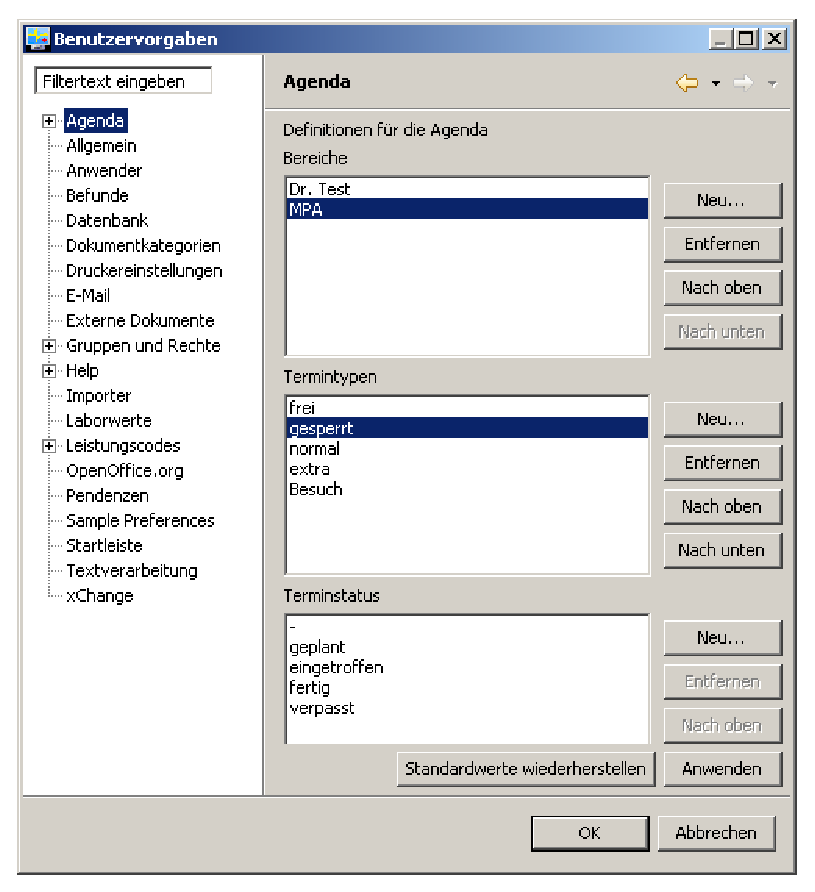
\includegraphics{images/settings1}

Dans la partie supérieure  \textit{Zone d'utilisateur} \index{Agenda!Zone d'utilisateur} vous pouvez définir combien et quelles agendas peuvent être gérées parallèlement. Il peut s'agir par exemple d'une agenda pour chaque médecin d'un
\index{cabinet de groupe} cabinet de groupe, ou des agendas pour des différentes ressources comme par exemple le médecin, ECG, Laboratoire, Ergométrie etc.
La quantité et le titre des 'zones d'utilisateur' dépend entièrement des besoins spécifiques de votre cabinet médical.

En dessous vous trouvez \textit{type de rendez-vous} \index{Agenda!type de rendez-vous}. Dans cette rubrique vous définissez quels types de rendez-vous sont à gérer par l'agenda dans votre cabinet. Un 'type de RDV' peut être toute sorte d'inscription qui se fera dans l'agenda. Par exemple aussi des  \textit{colloques avec l'équipe},  \textit{Acupuncture},  \textit{Check-Up},  \textit{Formation}  etc. Les 'types de RDV' seront affichés plus tard de façon individuelle et peuvent suivre des horaires différents.  Les deux premières inscriptions , 'libre' et 'réservé', doivent être introduits avec cette signification et dans cette séquence mais peuvent aussi être nommé différemment (par ex. \textit{vide}  et \textit{bloqué}). Les autres lignes vous pouvez nommer de façon arbitraire et il peut y avoir autant que vous voulez.

Le champ tout en bas, \textit{état du rendez-vous}\index{Agenda!état du rendez-vous}, est également très dépendant de la réalité spécifique de votre cabinet médicale. Comme dans le cadre des 'types de RDV' les deux premières inscriptions sont fixes dans leur signification mais peuvent changer de nom, tandis que les autres inscriptions sont tout à fait libres. On pourrait introduire ici par ex.   \textit{annulé}, \textit{attend résultats labo}, \textit{attend médecin}  etc.

La prochaine page de réglage de l'agenda concerne les icônes \index{Agenda!icônes} par lesquels les différents types de rendez-vous peuvent être affichés. Vous arrivez aux icônes dans la liste gauche sous rubrique 'utilisateurs' - 'Agenda-icons'.

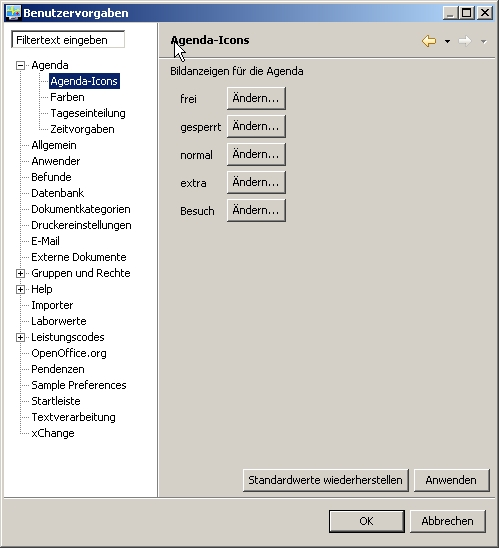
\includegraphics[width=3in]{images/settings2}

(Si en cliquant sur 'Agenda-icons' les 'types de RDV' que vous venez d'introduire ne s'affichent pas, il faut fermer Elexis et redémarrer pour qu'ils soient lus correctement.).
Cliquez sur le bouton  \textit{modifier} et choisissez une image dans le format  .*gif, *png oder *.ico .

La partie suivante concerne les couleurs d'affichage pour les 'types de RDV' et 'état du RDV' :

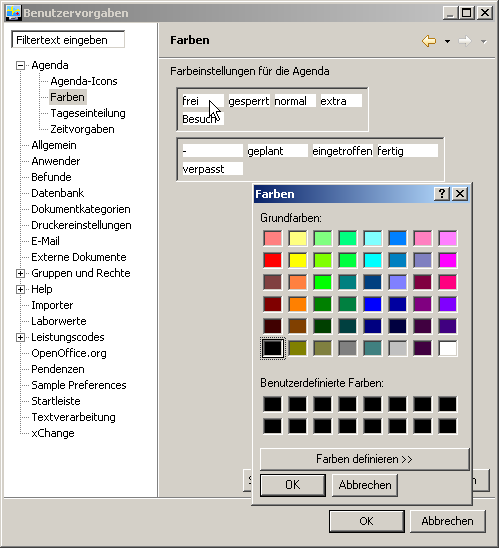
\includegraphics[width=3in]{images/settings3}

Choisissez sous 'utilisateur -couleurs' la couleur qui vous convient pour les différents champs des types de rendez-vous et d'état du RDV. Après un double-clic sur un champ vous pouvez choisir sa couleur.
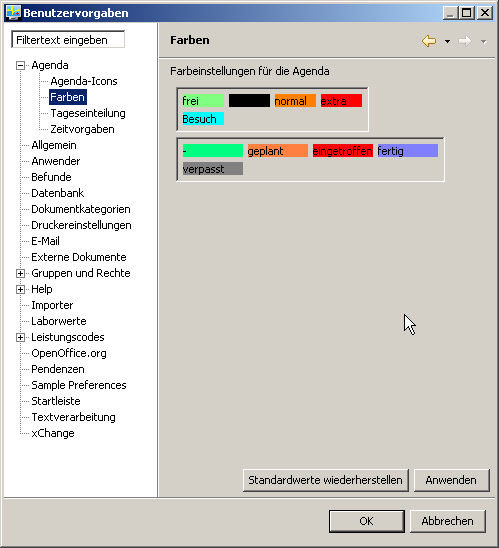
\includegraphics[width=3in]{images/settings4.png}


La ligne supérieure concerne les 'types de RDV'. Les couleurs affichées ici seront affichées dans le dialogue où on introduit les rendez-vous.
La ligne inférieure concerne 'l'état du RVD'. Les couleurs affichées ici seront affiché dans l'affichage normale de l'agenda.


La partie suivante du réglage de l'agenda concerne l'organisation de la journée \index{organisation de la journée}:

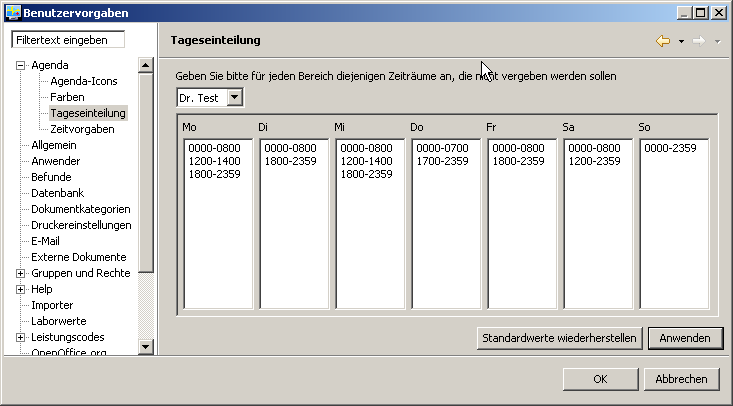
\includegraphics[width=3in]{images/settings5.png}
% settings5.png: 733x406 pixel, 96dpi, 19.39x10.74 cm, bb=0 0 550 304

Ici on peut régler pour chaque jour de la semaine les périodes qui seront de façon standard à disposition pour la planification. Ceci peut naturellement aussi être changé ultérieurement pour chaque jour mais ici il s'agit des préréglages approchés.

Choisissez en haut la 'zone d'utilisateur' souhaitée (par ex. un médecin du cabinet de groupe) et introduisez ici le début et la fin des périodes qui ne sont pas à disposition pour la planification. Ces plages de temps seront ensuite occupé par le 'type de RDV' \textit{bloqué} bloqué. Vous pouvez introduire des périodes de ce genre ad libitum pour chaque jour de la semaine.  \index{jour de la semaine}.

La dernière partie du réglage de l'agenda concerne le réglage du temps à programmer pour chaque 'type de RDV' :

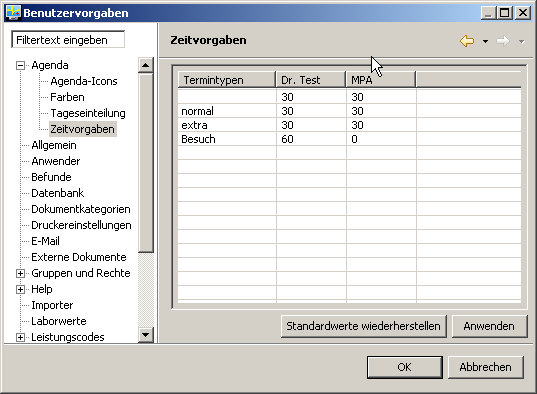
\includegraphics[width=3in]{images/settings6.png}
% settings6.png: 537x394 pixel, 96dpi, 14.21x10.42 cm, bb=0 0 403 295

Ici vous voyez pour chaque 'zone d'utilisateur' et chaque 'type de RDV' une possibilité de fixer le temps à programmer . Vous pouvez changer chaque champ en cliquant dessus et en écrivant par-dessus. L'agenda consacrera de façon standardisé le temps fixé pour ce type de RDV mais celui pourra être adapté manuellement si nécessaire. Si vous introduisez à un endroit 0, le type de RDV ne sera pas disponible pour cette 'zone d'utilisateur'. La ligne supérieure est le temps standard qui est toujours appliqué si le système ne trouve pas une autre durée spécifique.
En outre vous pouvez faire quelques réglages pour imprimer des cartes de rendez-vous. Ces réglages vous pouvez trouver sous \textit{impression}\index{Agenda!impression}.

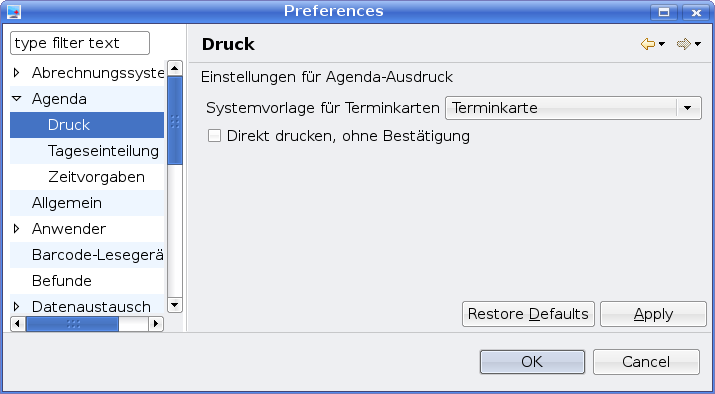
\includegraphics[width=3in]{images/settings-agenda-druck1.png}

Le modèle standard pour l'impression des cartes pour rendez-vous s'appelle  \textit{carte RDV}. Vous pouvez choisir un autre modèle système quelconque. Les heures du rendez-vous seront intégrés dans la variable
\textit{[rendez-vous]}.

Lors de l'impression de la carte RDV une fenêtre s'ouvre qui montre un aperçu de la carte RDV. Vous pouvez imprimer la carte RDV depuis le traitement de texte.
Si vous voulez que la carte RDV soit imprimée directement sur l'imprimante, marquez
\textit{imprimer directement}. Vous pouvez ensuite choisir l'imprimante et de façon optionnelle le bac de l'imprimante en question. Si vous ne choisissez pas de bac , le bac mémorisé dans le modèle système ou le bac standard de l'imprimante séléctionnée sera utilisé.

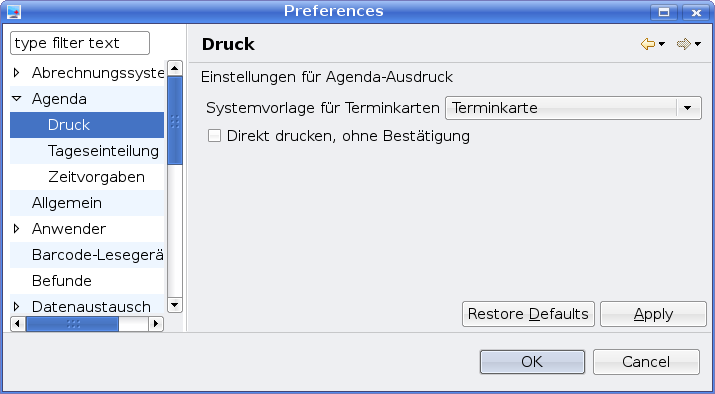
\includegraphics[width=3in]{images/settings-agenda-druck1.png}

Vous venez de finir la configuration de l'agenda. Cliquez sur la touche \textit{OK} et fermez Elexis. A partir du prochain démarrage du logiciel, les nouveaux réglages seront à disposition.

Les prochaines pages ont pour but de vous montrer l'utilisation de l'agenda.

\subsection{Utilisation de l'agenda}

La 'View-Agenda'  (Fig. \ref{fig:agenda1}) n'est normalement pas affichée.  Pour la visualiser choisissez dans le menu
 \textbf{fenêtre-view-autres}, tapez dans le champ de filtre en haut  \textit{agenda}, choisissez l'agenda et cliquez  \textit{OK}. Tirez ensuite la fenêtre de l'agenda \index{agenda-fenêtre} dans la position souhaitée de la perspective comme c'était décrit sous \textit{premiers pas} \ref{tour:customize} à la page \pageref{tour:customize}.
\begin{wrapfigure}[23]{L}{3in}
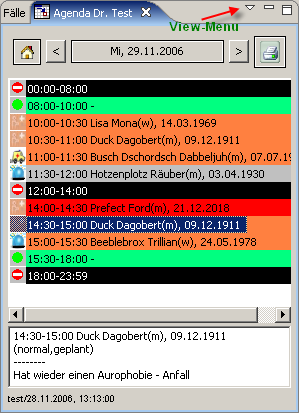
\includegraphics[width=3in]{images/use2.png}
\caption{Agenda-view standard}\label{fig:agenda1}
\end{wrapfigure}
Dans la partie à droite vous pouvez régler la date. Si vous cliquez sur le bouton 'aujourd'hui'vous arrivez au jour actuel.
Si vous cliquez sur les flèches vous pouvez avancer ou rétrocéder un mois et si vous cliquez sur les flèches doubles, vous pouvez avancer ou rétrocéder une année. Pour choisir une date spécifique cliquez directement dessus. Si vous cliquez sur le triangle en haut à droite, vous ouvrez le 'view-menu' dans lequel vous pouvez choisir la 'zone d'utilisateur' que vous voulez afficher et les limites des journées réglables ici individuellement.

Dans le secteur principale vous pouvez voir les inscriptions de l'agenda avec les couleurs et icônes que vous avez défini pour les différents types de rendez-vous. Les périodes libres sont en couleur verte. Prenez en considération que dans cette agenda la durée des périodes n'est pas proportionnel à leur espace visualisé. Au début il faut s'habituer un peu mais ceci s'est avéré très utile car par la suite on peut afficher toute la journée dans un espace relativement petit.

\medskip

Dans l'espace en bas à droite vous voyez des informations supplémentaires qui concernent le rendez-vous marqué actuellement.

\bigskip

Si vous double-cliquez sur une plage libre, vous pouvez introduire un nouveau rendez-vous et si vous double-cliquez sur un rendez-vous déjà donné vous pouvez le modifier. Dans les deux cas la boîte de dialogue s'ouvre Fig. \ref{fig:termineingabe}.

\begin{figure}[ht]
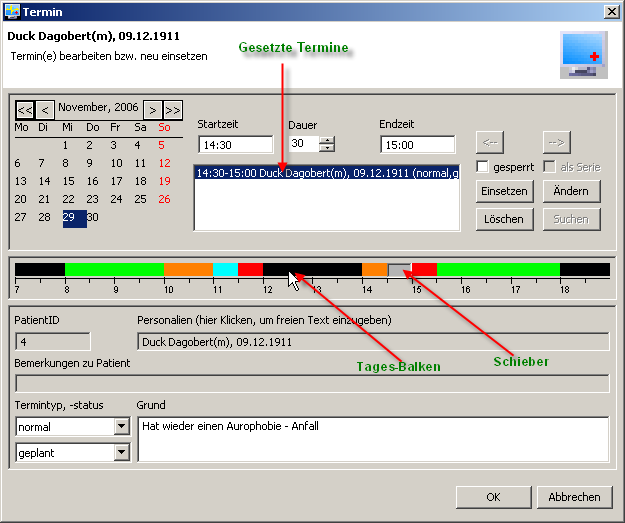
\includegraphics[width=5in]{images/use4.png}
% use4.png: 625x523 pixel, 96dpi, 16.53x13.84 cm, bb=0 0 469 392
\caption{Termineingabe-Dialog}\label{fig:termineingabe}
\end{figure}
La boîte de dialogue est assez complexe et contient des multiples plages :

\begin{itemize}
 \item En haut à gauche se trouve un calendrier qui vous permet de choisir aussi une autre journée.
\item En haut au milieu se trouvent les endroits où on introduit l'heure du début et l'heure de fin de la consultation de même que la durée de la consultation.
\item  En dessous vous trouvez la liste des rendez-vous où vous pouvez facilement voir quel
rendez-vous on avait déjà donné. (on peut fixer un ou plusieurs rendez-vous parallèlement).

\item En haut à droit vous trouvez la checkbox  \textit{verouillé}, ce qui bloque toute modification ultérieure du rendez-vous.
\item  En dessous vous trouvez le bouton pour  \textit{placer un rendez-vous}. Vous pouvez après avoir placé un rendez-vous choisir une autre date ou autre heure pour introduire un rendez-vous supplémentaire. (Si vous voulez introduire qu'un seul rendez-vous, vous pouvez cliquer directement sur 'OK'.
\item Au milieu vous trouvez la \textit{barre de la journée}, qui démontre l'organisation de la journée actuellement affichée. Les couleurs correspondent au types de consultations que vous avez défini pour les différents types de rendez-vous dans la configuration. Le curseur gris symbolise la période actuellement choisi. A l'aide de la souris vous pouvez placer ce curseur où vous voulez.
\item En dessous de la barre de la journée vous trouvez l'affichage horaire dont la trame peut être adaptée à vos besoins en cliquant dessus. Pour choisir l'heure pour une consultation vous déplacez le curseur sur la barre de la journée.


\item "	En dessous on trouve les coordonnées du patient séléctionné de même que le type et l'état du rendez-vous en question . Si vous ne voulez pas introduire un nom de patient mais un texte libre vous pouvez l'introduire dans le champ  \textit{identité}.
\end{itemize}

En cliquant sur ok l rendez-vous est introduit et le dialogue se ferme.


Si vous cliquez avec la touche droite sur un rendez-vous un menu contextuel s'ouvre dans lequel vous pouvez changer plusieurs détails concernant ce rendez-vous.

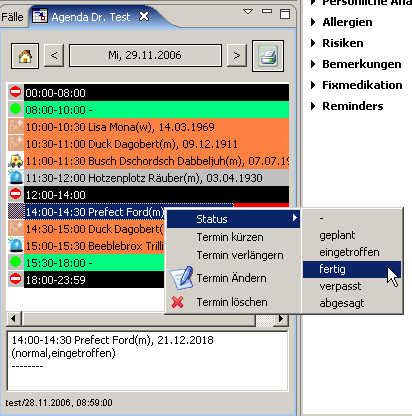
\includegraphics[width=4in]{images/use5.png}
% use5.png: 412x416 pixel, 96dpi, 10.90x11.01 cm, bb=0 0 309 312

Le plus important dans ce menu contextuel semble être \index{les changements de l'état du rendez-vous}: Puisqu'un tel changement se reproduit sur tout les ordinateurs branchés sur le réseau, ceci permet de constater sur n'importe quel poste de travail si par exemple le patient est \textit{arrivé}.

Si vous voulez changer pour une seule journée les périodes réservées vous pouvez le faire en choisissant dans le 'View-menu' (triangle à droite en haut)  \textit{les limitations de la journée}. Le champ de dialogue suivant se montre :

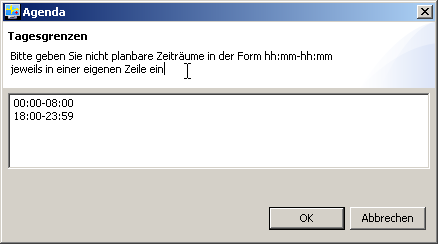
\includegraphics[width=3in]{images/use3.png}
% use3.png: 438x244 pixel, 96dpi, 11.59x6.46 cm, bb=0 0 328 183

Ici vous pouvez fixer les périodes réservées (bloquées) pour la journée actuelle comme décrit dans le chapitre configuration.

\subsubsection{Plusieurs agendas en même temps}
Vous pouvez sans problème laisser afficher plusieurs fenêtres d'agenda simultanément par exemple pour des différentes 'zones d'utilisateurs' ou des différentes journées.
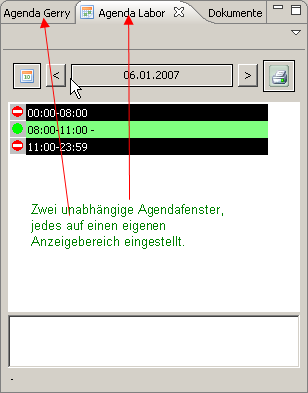
\includegraphics[width=3in]{images/agendamulti.png}
% agendamulti.png: 308x393 pixel, 96dpi, 8.15x10.40 cm, bb=0 0 231 295

\subsubsection{Fenêtre agrandie}

Votre assistante médicale aimerait peut être avoir sur son écran une agenda qui donne plus d'informations en même temps. Utilisez pour ceci la 'View' :  \textit{Agenda - grande}:

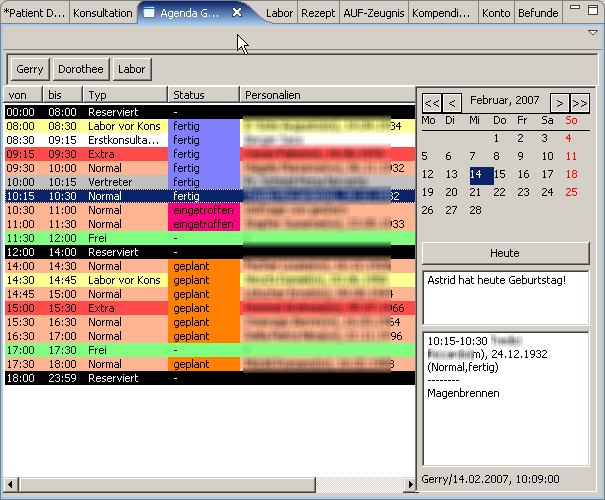
\includegraphics[width=5in]{images/agenda2.png}
% agenda2.png: 605x500 pixel, 96dpi, 16.01x13.23 cm, bb=0 0 454 375

Comme vous voyez tout les informations importantes peuvent être affichées de façon synoptique. Les fonctions expliquées de l'agenda restent par contre les mêmes. Si vous voulez vous pouvez naturellement aussi utiliser les deux 'views' de l'agenda simultanément.

\subsubsection{Imprimer des cartes de rendez-vous}

Dans le 'View-menu' (triangle à droite en haut) de l'agenda vous pouvez sélectionner \textit{imprimer carte de rendez-vous} pour le patient spécifique. Le style correspondant s'appelle \textit{carte de rendez-vous}.
Des informations plus détaillées pour la configuration vous trouvez ci-dessus.

Lors de l'impression d'une carte de rendez-vous apparaît une fenêtre avec la carte de rendez-vous préparée. Vous pouvez imprimer cette carte depuis le logiciel de traitement de texte et vous pouvez fermer cette fenêtre après avoir cliqué sur \textit{OK} ou \textit{Annuler}.

